\begin{figure}[t!]
\centering
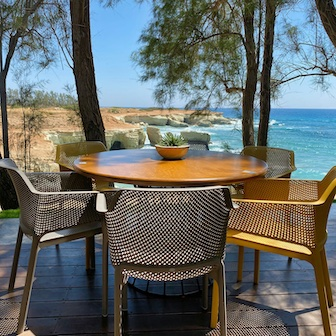
\includegraphics[width=0.2475\linewidth]{figures/shapenet/rw/0_in.jpg}\hfill
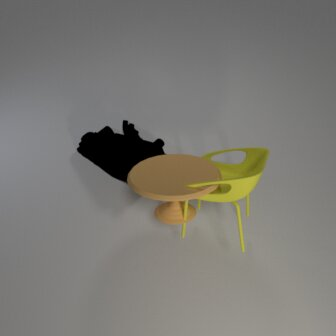
\includegraphics[width=0.2475\linewidth]{figures/shapenet/rw/0_out.jpg}\hfill
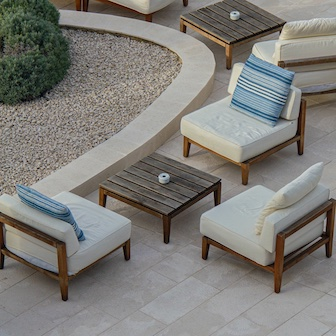
\includegraphics[width=0.2475\linewidth]{figures/shapenet/rw/1_in.jpg}\hfill
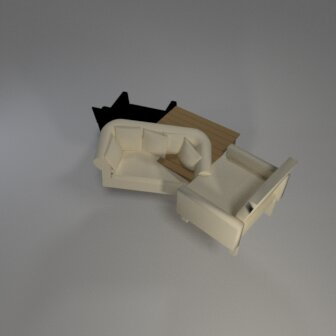
\includegraphics[width=0.2475\linewidth]{figures/shapenet/rw/1_out.jpg}
\caption{\textbf{Real-World ShapeNet 6-DoF Samples.} (\cref{sssec:scene_6dof}) 
Real-world sample reconstructions from the ShapeNet 6-Dof pose-estimation experiment.
We observe that the model is sensitive to OOD camera configurations.
During data generation, the camera is assigned a random pitch and radius, with its optical axis fixed passing through the global origin.
As such, we find that the model learns the bias and is limited by the expressivity of the training-data-generation framework, and, while it effectively interpolates values, it struggles to extrapolate outside of the camera configurations on which it was trained on.
We observe that the model is still, however, often able to identify the first few most-salient objects in the scene and produce meaningful assets (the first two in each of these samples being the rightmost chair then the table) before attempting to explain background features.
}
\label{fig:scene_6dof_rw_samples}
\end{figure}